\begin{frame}{Tổng quan các dịch vụ}
\begin{figure}[H]
\centering
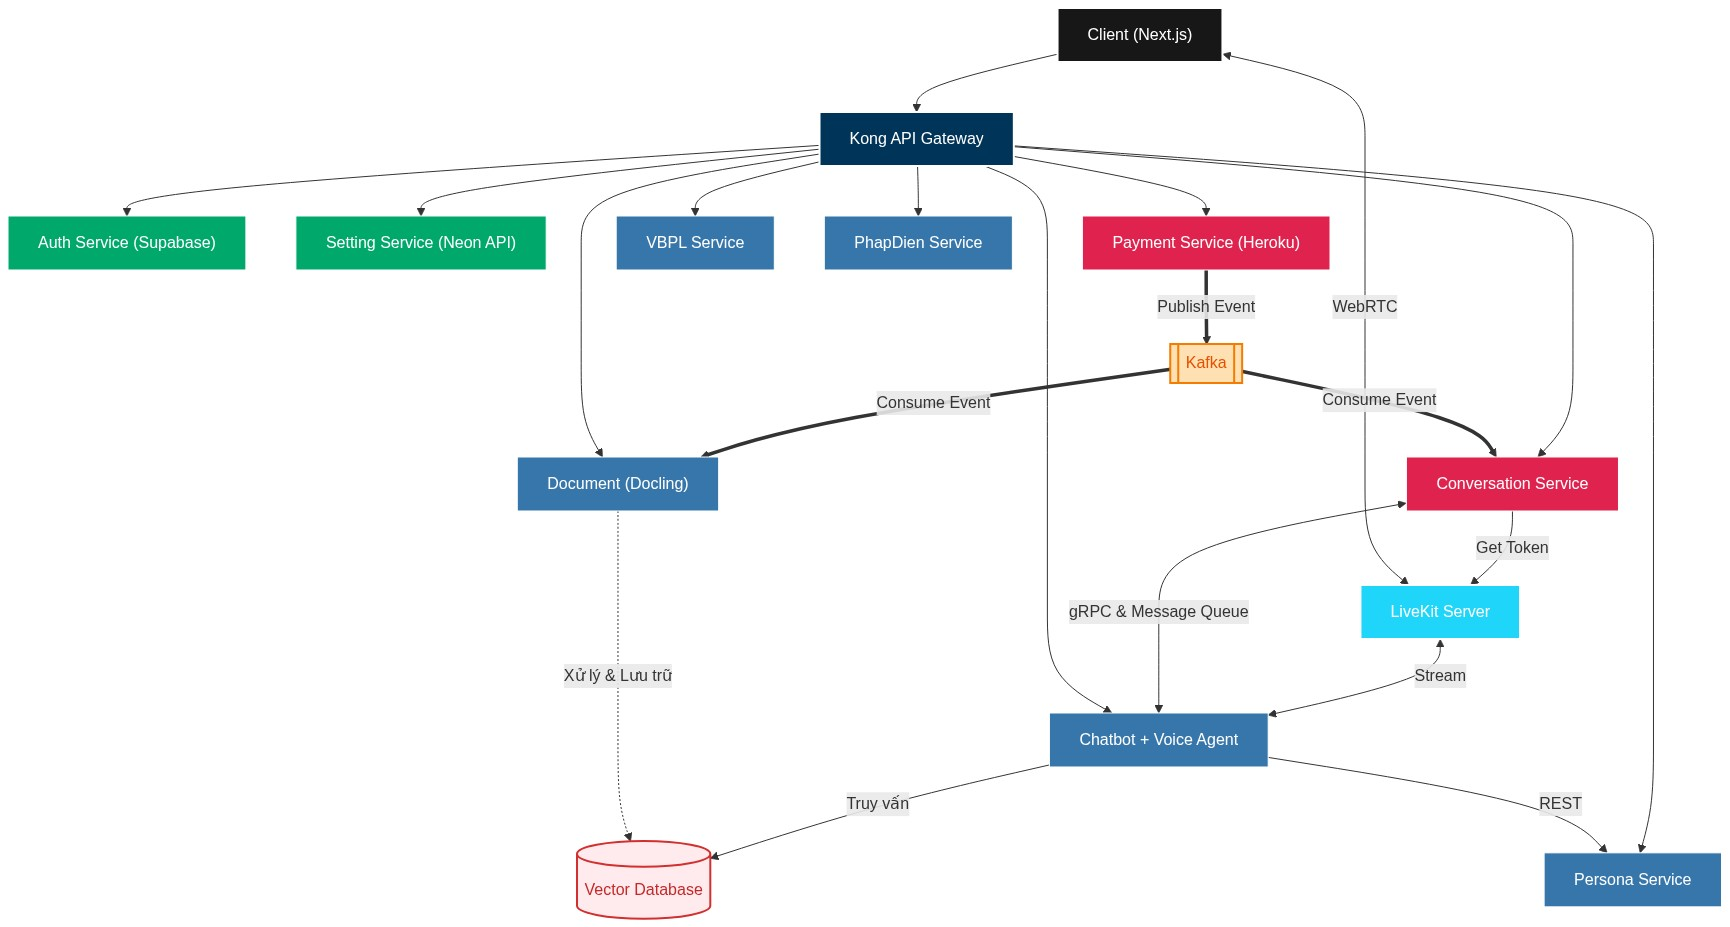
\includegraphics[width=\linewidth,height=0.99\textheight,keepaspectratio]{pictures/MSA.png}
\caption{Tổng quan các dịch vụ của dự án}
\end{figure}

\note{

Do khối lượng công việc AI
xử lý phức tạp và tốn kém 

Hệ thống sử dụng kiến trúc Microservice

giúp
 chia nhỏ hệ thống lớn  thành các dịch vụ nhỏ


 
Giúp Hệ thống tăng khả năng chịu lỗi

nếu dịch vụ  cài đặt bị  cash => thì dịch vụ đăng nhập thanh toán vẫn hoạt động 

% Ngôn ngữ khác nhau

% rủi ro bảo mật pháp luật
% mfa chặn hacker

% Vbpl và pháp điển thực hiện thống kê dữ liệu đang có trong db

% Auth xác thực người dùng tận dụng supabase setting dùng rest api lưu key và value

% Payment không tìm thấy hỗ trợ . Tự phát triển và tự triển khai trên heroku

Sơ đồ tổng quan về kiến trúc các vi dịch vụ được triển khai
trong dự án này.
Hệ thống được chia thành nhiều dịch vụ chuyên biệt như:

Auth Service (xác thực), Document Service (quản lý tài liệu),
Conversation Service (quản lý trò chuyện), Chatbot Service (trí tuệ nhân tạo)

và Payment Service (thanh toán).

Các dịch vụ này giao tiếp với nhau qua gRPC, REST API hoặc thông điệp bất đồng bộ qua Kafka/RabbitMQ.
}
\end{frame}
